\documentclass[runningheads]{llncs}
\usepackage{makeidx}  % allows for indexgeneration

%\usepackage{mathptmx}
\usepackage[scaled=0.91]{helvet}
\usepackage{courier}

%\usepackage[nocompress]{cite}
\usepackage{graphicx}
\graphicspath{{figures/}}
\usepackage[caption=false,font=footnotesize]{subfig}
%\usepackage{algorithmic}
%\usepackage[plain]{algorithm}
%\usepackage{amsmath,amssymb}

\usepackage{tabularx}

\usepackage[vlined,boxed,commentsnumbered]{algorithm2e}
\usepackage{wrapfig}

\usepackage[usenames,dvipsnames,svgnames,table]{xcolor}
\usepackage[obeyspaces]{url}
\urlstyle{sf}
\usepackage[breaklinks,colorlinks,linkcolor=DarkGreen,citecolor=DarkRed,urlcolor=white!0!blue!99]{hyperref}

\usepackage{comment}
\usepackage[vlined,boxed,commentsnumbered]{algorithm2e}
\usepackage{multirow}
\usepackage{hhline}

\hyphenation{per-for-man-ce}

\newcommand{\cre}[1]{\textcolor{red}{#1}}
\newcommand{\ignore}[1]{} 
\newcommand{\blasrout}[1]{\textbf{\texttt{#1}}}

\def\normo#1{\|#1\|_{\infty}}

\def\fqp{\texttt{FP128}\xspace}
\def\fdp{\texttt{FP64}\xspace}
\def\fsp{\texttt{FP32}\xspace}
\def\fhp{\texttt{FP16}\xspace}
\def\fhtp{\texttt{FP16-TC}\xspace}
\def\ir{\texttt{IR}\xspace}
\def\irgm{\texttt{IRGM}\xspace}

\def\fspir{\texttt{FP32 IR}\xspace}
\def\fhpir{\texttt{FP16 IR}\xspace}
\def\fhtpir{\texttt{FP16-TC IR}\xspace}
\def\fspirgm{\texttt{FP32 IRGM}\xspace}
\def\fhpirgm{\texttt{FP16 IRGM}\xspace}
\def\fhtpirgm{\texttt{FP16-TC IRGM}\xspace}

\usepackage{xspace}
\newcommand{\asgard}{ASGarD\xspace}
\newcommand{\magma}{MAGMA\xspace}

\begin{document}

% propose titles
\title{Boosting Performance of Physics Simulations up to $4\times$ through Mixed-precision Solvers	for GPU Tensor Cores
%\thanks{This research was partially supported by the National Science Foundation under Grants OCI-1032815, ACI-1339822, and DOE under Grants DE-SC0004983 and DE-SC0010042, and Intel Corporation.}
}
\titlerunning{Boosting Performance through Mixed-precision Solvers}
\toctitle{Boosting Performance through Mixed-precision Solvers}

% Double blind - edit but leave in comment for now
\begin{comment}
\author{Azzam Haidar\inst{1}  \and David Green\inst{3}, Stanimire Tomov\inst{2}, Ed D'Azevedo\inst{3}, Wael Elwasif\inst{3}, Graham Lopez\inst{3}, Tyler McDaniel\inst{3}, Lin Mu\inst{3}\and \\ Jack Dongarra\inst{2,3,4}}
\authorrunning{Haidar, Green, Tomov, D'Azevedo, Elwasif, Lopez, McDaniel, Mu, Dongarra}
\tocauthor{Haidar, Green, Tomov, D'Azevedo, Elwasif, Lopez, McDaniel, Mu, Dongarra}
\institute{NVIDIA USA, \and University of Tennessee, USA \and Oak Ridge National Laboratory, USA \and University of Manchester, UK}
\end{comment}

\maketitle

\begin{abstract}
While many scientific computing applications require 64-bit
floating-point (FP64) arithmetic and accuracy, commodity 
hardware like GPUs now support FP16 operations
that are up to $16\times$ faster than FP64. This raises a
significant interest in the development of mixed-precision 
methods that can boost significantly performance
while maintaining FP64 accuracy. We present a mixed-precision
methodology that uses a combination of FP16, FP32, and FP64 operations to achieve this for real-world applications. 
Namely, the developments are for a scientific application 
using  a Discontinuous-Galerkin (DG) 
finite element solver based on a hierarchical sparse-grid
discretization. As with any other DG solver, an implicit time
advance (here Backward Euler) requires a matrix factorization. 
The new FP16-FP32-FP64 solver uses a mixed FP16-FP32 precision
factorization and a FP64 iterative process, preconditined with 
the mixed-precision factorization, that yields FP64 accuracy.  
Results on latest GPUs are presented, illustrating 
a significant, up to $4\times$, speedup and FP64 accuracy.
\end{abstract}
\section{Introduction}\label{sec:intro}
\section{Related work}\label{sec:related}

% Start with text from SC18 paper
Iterative refinement is a well-established technique that dates back to
Wilkinson in the 1940s. The idea is to improve the computed solution of a
linear system by solving a correction equation and adding the
correction to the original solution; see Wilkinson \cite{Wilkinson_1963},
Moler~\cite{Moler_1967_jacm}, Stewart~\cite{Stewart_1973},
Demmel~\cite{Demmel_1997})
and, for a comprehensive treatment, Higham~\cite[Chap.~12]{Higham_2002}.
In iterative refinement, the three tasks (original solve/factorization,
residual computation, and correction equation solve) can be done in the
same precision (fixed precision) or in different precisions (mixed
precision). Fixed precision iterative refinement was analyzed by
Skeel~\cite{Skeel80} for an LU solver and extended by
Higham~\cite{Higham1991}, \cite{high97i} for a general solver. In the 2000s, motivated by
processors equipped with \fsp speed 2$\times$ that of \fdp, mixed precision
iterative refinement---with the LU factorization done in \fsp and
everything else done in \fdp---was explored
in~\cite{Langou_2006_sc,Buttari_2007_sc}.

Replacing the direct triangular solves of the correction equation with an
iterative method,
as suggested in \cite{carson2017new} in a mixed precision context,
leads to ``nesting'' of two iterative methods, which in general
are called ``inner--outer'' iterations, the latter having been studied both
theoretically and
computationally~\cite{golub00inexact,saad91flexible,flexible-inner-outer},
including in mixed-precision computation
scenarios~\cite{BaboulinBDKLLLT09}.
Recently, Carson and Higham~\cite{carson2017accelerating,carson2017new}
analyzed the convergence property of a three precision iterative refinement scheme
(factorization precision, working precision, residual precision) and concluded that
if the condition number of $A$ is not too large,
$\kappa_\infty(A) = \normo{A}\normo{A^{-1}}<10^4$,
then using
\fhp for the $O(n^3)$ portion (the LU factorization)
and (\fsp, \fdp) or (\fdp, \fqp)
as the (working, residual) precision for
the $O(n^2)$ portion (refinement loop),
one can expect to achieve
forward error and
backward error  on the order of $10^{-8}$ and $10^{-16}$ respectively.
%                                                     
We note that, if $\hat{x}$ is the solution of $Ax=b$
the forward error is defined by $\Vert \hat{x} - x \Vert_\infty/\Vert x \Vert_\infty$
and the backward error is defined by 
$\Vert r \Vert_{2} / \Vert A \Vert_{2} \Vert \hat{x} \Vert_{2}$ where $r=b-A\hat{x}$.
%                                                           
The same study also showed that when using the generalized minimal residual
(GMRES) method preconditioned by the \fhp LU factorization
as the refinement procedure, the
constraint on the condition number can be relaxed to be
$\kappa_\infty(A)<10^8$ when the (working, residual) precision is (\fsp, \fdp)
and to $10^{12}$ when the (working, residual) precision is (\fdp, \fqp).

An investigation of similar iterative refinement methods
on earlier generations of GPUs can be found in~\cite{Haidar2017}.
With the
announcement of NVIDIA's V100 Tensor Cores. which improve
numerical precision and speed for \fhp, it is our
intention to comprehensively investigate how the V100 opens a
new world of opportunities in matrix computations.

Recently~\cite{Haidar2018}
\section{Physics Application}
\label{sec:physics}
%
% Motivation for application to this code
%
With the recent availability of the Summit supercomputer at the Oak Ridge National Laboratory Leadership Computing Facility (OLCF) and its Tensor core enabled NVIDIA Volta GPUs, there is significant interest from the scientific community in methods and libraries which can enable efficient utilization of the extra compute capacity the Tensor cores represent. Here we partner with the developers of the \asgard \cite{} application as their GPU enabled code relies on the factorization of a close-to-dense double precision matrix at each time step, such that our new \magma capability could be demonstrated within a real application. 
%
% Brief details of the application method
The \asgard code is a Discontinuous-Galerkin (DG) finite element solver based on a hierarchical sparse-grid discretization. As with any other DG solver, for an implicit time advance (here Backward Euler) requires a matrix factorization. For this study we apply \asgard to the nonlinear Vlasov-Poisson system of equations such that the system matrix must be constructed and factorized at each time step. And what makes \asgard unique, and well suited to application of our new FP16 solver, is that the sparse-grid discretization results in much smaller, yet denser system matrices than the typical sparse matrices of the DG method. As such, dense matrix operations such as that which we apply here are of direct use in accelerating the code. 
%
\subsection*{Two Stream Instability Benchmark}
% Equation set being solved.
The system under consideration is the Vlasov-Poisson equation set for a single charged species with a neutralizing uniform background charge, i.e., electrons within a stationary ion background plasma (cf. the $1$ in Eq.~\ref{eq:poisson}). 
\begin{equation}
    \frac{\partial f}{\partial t}+v\frac{\partial f}{\partial x}+E\left(x,t\right)\frac{\partial f}{\partial v}
    \label{eq:vlasov}
\end{equation}
%
\begin{equation}
-\frac{\partial^2\phi}{\partial x^2}=\rho-1
    \label{eq:poisson}
\end{equation}
%
\begin{equation}
E\left(x,t\right)=-\frac{\partial\phi}{\partial x}
    \label{eq:E}
\end{equation}
where $\rho\left(x,t\right)=\int_v f\left(x,v,t\right) dv$ denotes the electron density as a function of space $x$, velocity $v$ and time $t$. The particular scenario we apply \asgard to here is the ``two stream instability'' benchmark which describes an electrostatic instability which forms as a result of two counter propagating charged particle beams. This scenario is described by the initial conditions $f\left(0,x,t\right)=f_{\mathrm{TSI}}\left(v\right)\left(1+A \cos\left(k x\right)\right)$, 
$x\in\left[0,13\right]$, $v\in\left[-5,5\right]$, 
where $A=0.05$, $k=2/13$, 
and 
$f_{\mathrm{TSI}}
\left(v\right)
=
\frac{1}{2 v_t \sqrt{2\pi}}
\left(
\exp\left(-\frac{\left|u+v\right|^2}{2v_t^2}\right)
+
\exp\left(-\frac{\left|u-v\right|^2}{2v_t^2}\right)
\right)$, where $u=0.99$ and $v_t=0.3$. We note that since the coefficient of the LHS of Eq.~\ref{eq:poisson} do not vary in time, that the Poisson factor can be done outside the time loop, such that only an equation for the implicit time advance of Eq.~\ref{eq:vlasov} must be inverted at each time step, with the coupling between the two being done explicitly. 
\begin{figure}
    \centering
    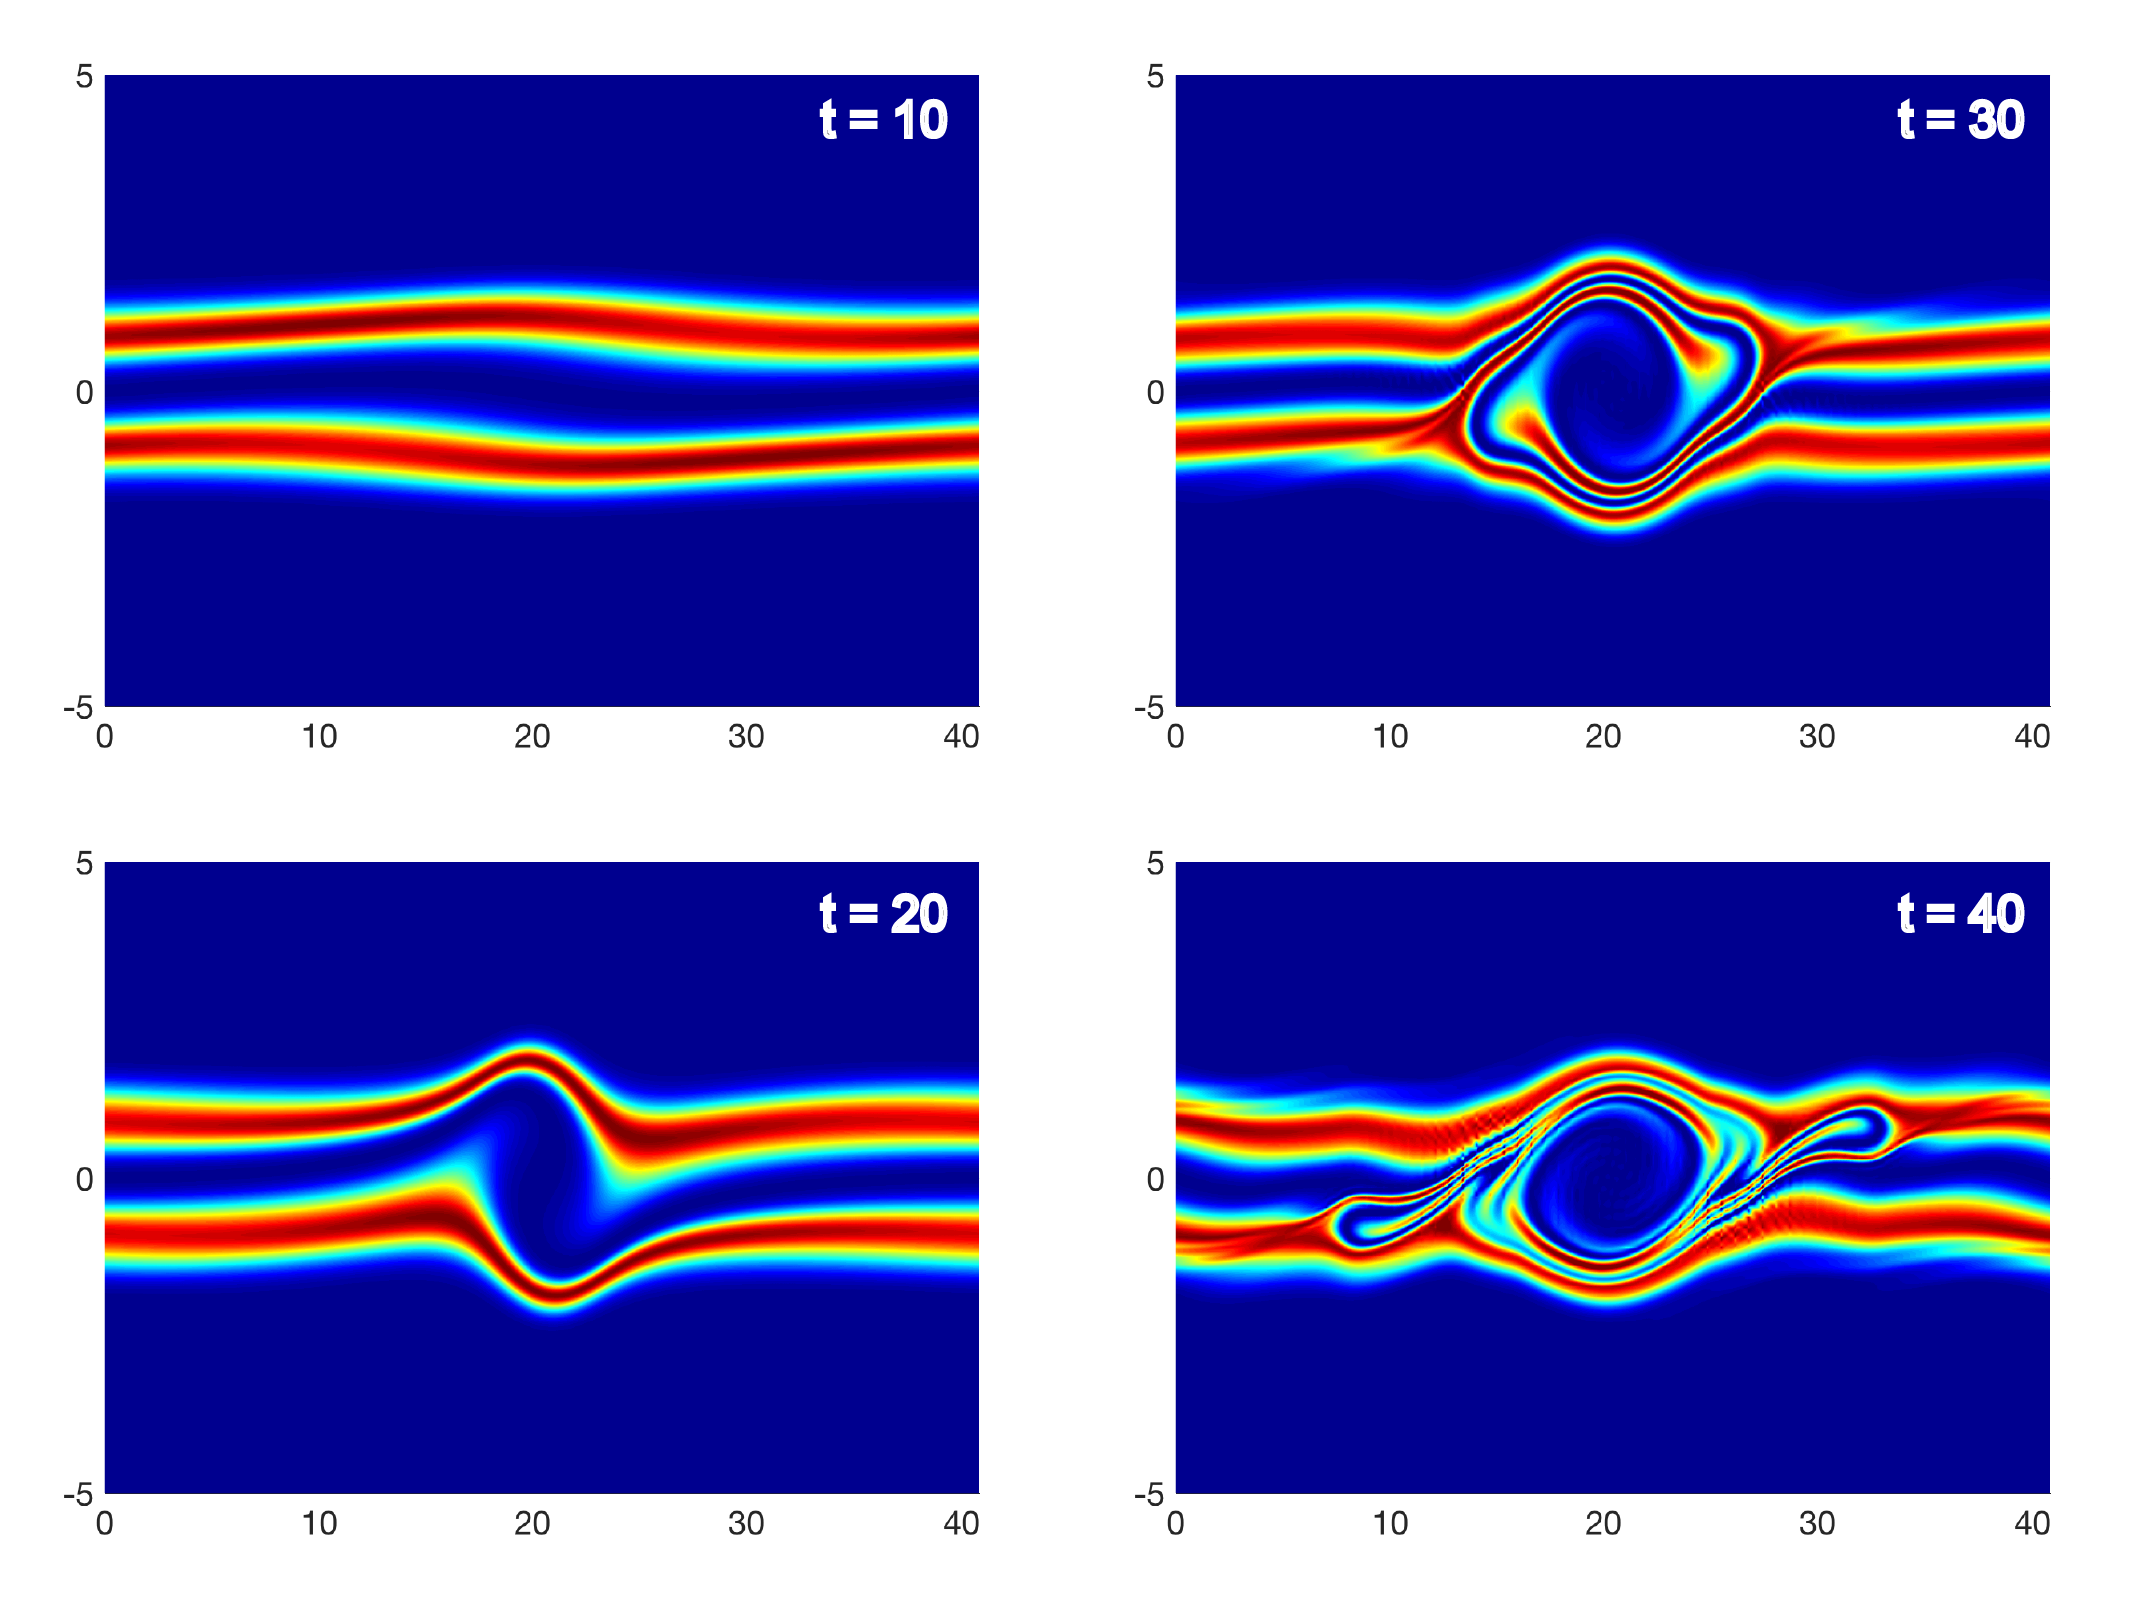
\includegraphics[width=\textwidth]{fp16_fk6d/figures/two-stream-01.png}
    \caption{Phase space ($x$ horizontal, $v$ vertical) contours of the electron probability distribution function $f\left(x,v,t\right)$ as solutions to the two stream instability benchmark at times t=10,20,30,40. These were using the global Lax-Friedrich's choice of numerical flux in the DG method.}
    \label{fig:my_label}
\end{figure}
% Time discretization

% 
\section{Iterative Refinement Techniques}\label{sec:ir}
\cre{some text about iterative refinement that the factorization happen in low precision while the IR happen in FP16}

\section{Mixed-precision algorithms}\label{sec:mixedp}
\cre{
Here we will talk that basic FP16 LU will not work properly and for that we needed 
1- mixed precision factorization
2- tensor cores that does accumulation in FP32
}


\section{Algorithmic Advancements}\label{sec:mixedp}
\cre{
Here we can talk about classical versus GMRES based refinement and say that for FP16 classical may fail while GMRES will recover and I can add a graph about this}


\section{Performance results}\label{sec:perf}
\section{Conclusions and Future Directions}\label{sec:concl}

% This is double blind - add acknowledgments but leave for now in comment
\begin{comment}
\section*{Acknowledgments}
This research was supported by the Exascale Computing Project
(17-SC-20-SC), a collaborative effort of the U.S. Department of Energy
Office of Science and the National Nuclear Security Administration. The
work was also partially supported by Nvidia and NSF grant No. OAC-1740250.
\end{comment}

%\bibliographystyle{plain}
\bibliographystyle{splncs04}
\bibliography{batched,magma,others,iter_ref,s7_mixed}

\end{document}


